% !TeX program = xelatex
% Needs XeLaTeX (Bengali examples). The bibliography uses Biber (Overleaf runs it automatically).
\documentclass[12pt]{report}

% Font: TeX Gyre Termes is a Times New Roman clone that ships with TeX Live and Overleaf.
% If you prefer the real Times New Roman on a local machine, change it to \setmainfont{Times New Roman}.
% Works with pdfLaTeX (Overleaf default) and with XeLaTeX/LuaLaTeX.
\usepackage{iftex}
\ifPDFTeX
  \usepackage[T1]{fontenc}
  \usepackage[utf8]{inputenc}
  \usepackage{tgtermes}
\else
  \usepackage{fontspec}
  \setmainfont{TeX Gyre Termes}
  % Bengali text for the examples: Noto Serif Bengali if installed, otherwise FreeSerif.
  \IfFontExistsTF{Noto Serif Bengali}%
    {\newfontfamily\bnfont[Script=Bengali]{Noto Serif Bengali}}%
    {\newfontfamily\bnfont[Script=Bengali]{FreeSerif}}
\fi
\ifPDFTeX
  \newcommand{\bn}[1]{\textit{[Bengali text: compile with XeLaTeX]}}
\else
  \newcommand{\bn}[1]{{\bnfont #1}}
\fi

\usepackage{graphicx}
\graphicspath{{figures/}{./}}
\usepackage{float}
\usepackage{amsmath,amssymb,amsfonts}
\usepackage{textcomp}
\usepackage[table]{xcolor}
\usepackage[hidelinks]{hyperref}
\usepackage{url}
\usepackage{ragged2e}
\usepackage{array,multirow}
\usepackage{booktabs}
\usepackage{enumitem}
\usepackage{tikz}
\usetikzlibrary{arrows.meta,positioning}
\usepackage[backend=biber,style=numeric,sorting=none]{biblatex}
\addbibresource{ref.bib}

\usepackage[parfill]{parskip}
\usepackage{geometry}
\usepackage{sectsty}
\chapterfont{\centering}

\geometry{
	paper=a4paper,
	top=1in,
	bottom=1in,
	left=1.2in,
	right=0.8in,
	headheight=0.75cm,
	footskip=1.5cm,
	headsep=0.75cm,
}
\linespread{1.5}

% ---------------------------------------------------------------------------
% Visible reminder for anything still to be filled in. Search the project for TODO before submitting.
\newcommand{\todo}[1]{\textbf{\textcolor{red}{[TODO: #1]}}}
% ---------------------------------------------------------------------------

\begin{document}

% ============================ TITLE PAGE ============================
\begin{titlepage}
	\centering
	
\includegraphics[height=4cm,width=4cm]{unilogo.png}\par
	\vspace{0.3cm}
	{\huge\bfseries Comilla University \par}
	\vspace{0.5cm}
	{\scshape\Large\bfseries A Retrieval-Augmented Bangla Question Answering System with a Fine-Tuned BanglaT5\par}
	\vspace{0.45cm}
	{\scshape\Large\bfseries A RESEARCH PROJECT REPORT \par}
	{\scshape\Large\bfseries \textit{Submitted By}\par}
	{\Large\textbf{Md MEHEDI HASAN PARVEZ}}\par
	{\Large{ID: 22408023}}\par
	\vspace{0.35cm}
	{\large\textbf{\textit{In Partial Fulfillment for the course Research Project of}}}\par
	{\Large\textbf{MASTER OF SCIENCE\\}}
	\vspace{0.1cm}
	{\large\textbf{IN }}
	{\large\textbf{DEPARTMENT OF COMPUTER SCIENCE AND ENGINEERING}\par}
	\vspace{0.45cm}
	{\Large\textbf{COMILLA UNIVERSITY , CUMILLA-3506}}\par
	\vspace{0.35cm}
	{\Large\bfseries November 2026\par}
\end{titlepage}

% ============================ CERTIFICATE ============================
\newpage
\pagenumbering{gobble}
\begin{center}
	\large\textbf{BONAFIDE CERTIFICATE}\\
\end{center}
\section*{}
This is to certify that this research project entitled
\textbf{``A Retrieval-Augmented Bangla Question Answering System with a Fine-Tuned BanglaT5''}
is submitted by \textbf{Md Mehedi Hasan Parvez}, who carried out the project work under my supervision. This is the bonafide work.
\\
\\

\begin{table}[h]
	\begin{tabular}{l@{\hspace{3cm}}l}
		{Signature} & {Signature} \\
		\\
		\ldots\ldots\ldots\ldots\ldots\ldots\ldots\ldots & \ldots\ldots\ldots\ldots\ldots\ldots\ldots\ldots \\
		Dr. Mahmudul Hasan & Md. Zahidur Rahman \\
		\textbf{Chairman of the Exam Committee} & \textbf{Supervisor} \\
		Associate Professor & Lecturer \\
		Department of CSE & Department of CSE \\
		Comilla University, Cumilla. & Comilla University, Cumilla. \\
	\end{tabular}
\end{table}

\pagenumbering{Roman}

% ============================ ABSTRACT ============================
\chapter*{Abstract}
\addcontentsline{toc}{chapter}{\numberline{}Abstract}
A small language model cannot store many facts, so a question about a particular text is better answered by searching a collection first and reading the best passage. This project builds a question-answering system of that kind for Bangla. The reader is BanglaT5, fine-tuned on the BanglaRQA dataset to answer from a passage, or to write nothing when the passage does not contain the answer. The knowledge base is the 3,000 Wikipedia passages of BanglaRQA, searched with BM25, with BGE-M3 dense retrieval, or with a hybrid of the two.

One trained model was tested on the 1,493 held-out questions, first with the correct passage and then with the top passage from each retriever. With the correct passage it reached an exact match of 59.9 and an F1 of 76.1, against 62.4 and 78.1 published for the same model type. It was slightly better than the published model on answerable questions and worse on unanswerable ones. On answerable questions, finding the passage with a retriever cost 4.1 exact-match points with BM25, 6.1 with the hybrid and 10.6 with dense retrieval, and the differences were statistically significant. Almost all of the loss came from questions for which the wrong passage was retrieved. Exact match also undercounts: with the correct passage 82\% of the answers reached an F1 of at least 0.5, while 56\% matched exactly. A small web page shows the system answering questions together with the passage it used.

In a hand-labelled sample of 40 wrong answers given with the correct passage, 78\% differed from the reference only in wording and a further 18\% were partly right; none gave a wrong value.

The study uses general Wikipedia text, one model size, one training run and a library of 3,000 passages, so the results describe this setting and need to be checked on other domains.

\medskip
\noindent\textbf{Keywords:} Bangla, question answering, retrieval-augmented generation, BanglaT5, BM25, dense retrieval, hybrid retrieval, unanswerable questions.


% ============================ ACKNOWLEDGEMENT ============================
\chapter*{Acknowledgement}
\addcontentsline{toc}{chapter}{\numberline{}Acknowledgements}
First and foremost, I thank the Almighty Allah for the health and determination that allowed me to complete this project.

\noindent I extend my sincere gratitude to my supervisor, \textbf{Md. Zahidur Rahman}, for the guidance, feedback and encouragement that shaped this work.

\noindent I thank the creators of the BanglaRQA dataset and of the BanglaT5 model for making them publicly available, and the maintainers of the open-source libraries used in this project.

\noindent Finally, I thank my family and friends for their constant support.

% ============================ CONTENTS ============================
\newpage
\renewcommand*\contentsname{Table of Contents}
\tableofcontents
\listoffigures
\listoftables
\pagenumbering{arabic}

\justifying

% ============================ CHAPTERS ============================
\chapter{Introduction}

\section{Background}

A question-answering (QA) system takes a question in natural language and returns an answer. For Bangla, a language with more than 200 million speakers, such systems are still much less developed than for English. Two things limit them. There are few large, well-annotated Bangla QA datasets, and the language models available for Bangla are small compared with the models used in English-language work.

A small language model has a further problem: it cannot store many facts. If it is asked about a person, a place or an event that it saw rarely or never during training, it either gives a wrong answer or makes one up. Making the model larger helps but is expensive, and the facts inside a model cannot be updated without training it again.

Retrieval-augmented generation (RAG) avoids both problems \cite{lewis2020rag}. The facts are kept in a separate document collection. When a question arrives, a retriever searches the collection and passes the best passage to the model together with the question. The model's job is then to read the passage and write the answer. The collection can be changed at any time without touching the model, and the passage that was used can be shown to the user as the source of the answer.

\section{Motivation}

This project asks what a Bangla RAG system built from open, small components can do. Three practical questions motivate it.

First, the model has to learn the skill of answering from a passage. BanglaT5 \cite{bhattacharjee2023banglat5} is pretrained on Bangla text but has no question-answering ability of its own, so it must be fine-tuned. Second, the retriever has to find the right passage before the model can use it. Keyword search and meaning-based search can behave differently on Bangla, because Bangla words appear in many inflected forms and embedding models are often trained mostly on other languages. Third, the system has to know when the collection does not contain the answer. A system that always produces an answer is less useful than one that says it cannot answer.

\section{Problem Statement}

Given a Bangla question and a collection of Bangla passages, the system must return the answer if the collection contains it and an empty answer if it does not. Existing work on the BanglaRQA dataset \cite{ekram2022banglarqa} measures how well a fine-tuned model reads a passage that is already known to be the correct one. In a real system the passage has to be found first, and an error in retrieval becomes an error in the answer. It is not known from the published results how much accuracy is lost at this step for Bangla, nor which retrieval method loses the least.

\section{Objectives}

The objectives of this project are to:
\begin{enumerate}
	\item fine-tune BanglaT5 on BanglaRQA so that it answers a question from a given passage, and answers with an empty string when the passage does not contain the answer;
	\item build a retrieval component over the 3,000 BanglaRQA passages with three methods: BM25, dense retrieval and a hybrid of the two;
	\item combine retrieval and the fine-tuned model into one question-answering pipeline;
	\item evaluate the pipeline on the held-out test questions with the metrics used by the dataset authors, and compare the three retrieval methods against each other and against the case where the correct passage is supplied;
	\item analyse where the remaining errors come from.
\end{enumerate}

\section{Scope and Limitations of the Study}

The knowledge base is the Wikipedia passages of BanglaRQA, so the system answers questions about the topics in that collection and not about arbitrary subjects. Only one model (BanglaT5, about 247 million parameters) is fine-tuned, once, and only one embedding model (BGE-M3) is used for dense retrieval. The retrievers are used as published and are not trained. The study does not include a comparison with large commercial language models. These choices keep the study small enough to repeat on a single GPU, and they define what the results can and cannot show.

\section{Functionality of the Proposed System}

A user types a Bangla question. The system searches the passage collection and selects the best-matching passage. It then gives the question and that passage to the fine-tuned BanglaT5 model, which writes a short answer. If the model judges that the passage does not contain the answer, it returns an empty answer. The passage is returned with the answer so that the user can check it.

\section{Contributions}

The contributions are:
\begin{itemize}
	\item a fine-tuned BanglaT5 question-answering model trained on BanglaRQA, with its training procedure documented;
	\item a retrieval-augmented pipeline for Bangla with three interchangeable retrievers;
	\item a controlled comparison of the three retrievers, measured both by how often they find the correct passage and by the accuracy of the final answers, with confidence intervals and paired significance tests;
	\item an analysis of how often an unanswerable question is handled correctly, and how much of the score on those questions depends on retrieval;
	\item an error analysis that separates retrieval failures from reading failures;
	\item a small web page that shows the answer together with the passage it was read from.
\end{itemize}

\section{Report Organization}

Chapter~2 reviews related work on Bangla QA, BanglaT5, retrieval-augmented generation and retrieval methods. Chapter~3 describes the dataset, the system and the evaluation. Chapter~4 reports the training results and the evaluation results, and discusses them. Chapter~5 concludes and lists limitations and future work.

\chapter{Literature Review}

This chapter reviews three areas: retrieval methods used in RAG, existing Bangla RAG and question-answering work, and the validation of LLM-based evaluators, including RAGAS. It ends with the gap this project addresses.

\section{Retrieval Methods for RAG}

\textbf{Keyword retrieval.} BM25 ranks passages by how often the query terms appear in them, adjusted for passage length and term rarity \cite{robertson2009bm25}. It needs no training and is a strong baseline, but it depends on how text is split into words. This matters for Bangla, where inflection and the way characters combine can split or merge tokens. This project tokenises on whitespace after removing punctuation, rather than on regular-expression word characters, which would split Bangla words at vowel signs.

\textbf{Dense retrieval.} Dense retrievers map the query and each passage to vectors and rank by similarity. BGE-M3 is a multilingual embedding model that supports long inputs and more than 100 languages \cite{chen2024bgem3}. Multilingual E5 is a comparable model family \cite{wang2024me5}. Sentence encoders tuned for similarity rather than retrieval, such as Bengali SBERT, may behave differently on retrieval tasks. The reviewed sources did not include a Bangla-specific comparison of these models, although indirect evidence from multilingual retrieval benchmarks suggests BGE-M3 and multilingual E5 are broadly comparable.

\textbf{Hybrid retrieval.} Hybrid methods combine the keyword and dense rankings. Reciprocal rank fusion (RRF) merges ranked lists by summing $1/(k+\text{rank})$ over the lists and needs no score calibration \cite{cormack2009rrf}. This project uses RRF with $k=60$.

\section{Bangla RAG and Question Answering}

\textbf{BanglaRQA.} BanglaRQA is a Bangla reading-comprehension dataset built on Wikipedia passages with several question and answer types \cite{ekram2022banglarqa}. It is used here as both the question source and the retrieval corpus.

\textbf{BanglaMedQA.} Work from the Islamic University of Technology benchmarks RAG strategies on Bangla medical multiple-choice questions, using a Class 12 biology textbook as the corpus, a Bengali sentence-embedding retriever and fixed chunking \cite{sultana2025banglamedqa}. It varies the RAG strategy (traditional, agentic, iterative and others) rather than the retrieval components. It also reports that strong generators already score highly without retrieval, which limits how much retrieval can add. The original plan for this project used the same textbook, but the text could not be obtained in time (Section~\ref{sec:domain}).

\textbf{Other Bangla RAG systems.} Several 2025--2026 preprints describe application-specific Bangla RAG systems, for example in legal, agricultural, diabetes-guideline and knowledge-base QA settings. At least two combine BM25 with BGE-M3 \cite{aich2026hybridragbn}. In the sources found, these report end-to-end results for one pipeline rather than a controlled comparison of retrieval components. \todo{Verify each of these preprints directly before citing more than this one, and run a Google Scholar / Semantic Scholar search for ``Bangla RAG'' ablations.}

\section{Evaluating Answers with LLM Judges}

\textbf{RAGAS.} The RAGAS framework defines reference-free metrics, including faithfulness (are the answer's claims supported by the retrieved context?) and answer relevancy (does the answer address the question?) \cite{es2023ragas}. In its original paper, agreement with human annotation was measured on a small English set; faithfulness agreed most (0.95), and answer relevance less (0.78).

\textbf{Multilingual validation.} MEMERAG meta-evaluates LLM judges for RAG on five languages (English, German, Spanish, French, Hindi) with expert annotation, and reports only moderate balanced accuracy on faithfulness; Bengali is not covered and all prompts were in English \cite{blandon2025memerag}. The closest direct precedent is work adapting RAGAS to Romanian and validating it against native-speaker annotation \cite{creanga2026romanian}. Beyond RAG, the Pariksha study compared human and LLM evaluators on ten Indic languages including Bengali, and found lower human--LLM agreement on direct assessment for Bengali than the cross-language average (Kendall's $\tau$ of 0.43 against 0.65) \cite{watts2024pariksha}.

\textbf{Limits of the evidence.} Evidence on RAGAS stability comes mostly from practitioner material rather than peer-reviewed studies. No guidance on the human sample size needed to validate a judge was found; the sample size here follows practical constraints and the confidence intervals reported in Chapter~4 show its precision.

\section{Research Gap}

Together, the reviewed work leaves two gaps that this project addresses on a small scale:
\begin{enumerate}
	\item no controlled comparison of no-retrieval, keyword, dense and hybrid retrieval with one fixed generator and prompt on a Bangla QA dataset was found;
	\item no validation of RAGAS faithfulness and answer-relevancy scores against human grades on Bangla RAG answers was found.
\end{enumerate}
Both statements rest on a web-based search and should be read as ``to the best of our knowledge''.

\chapter{Methodology}

\section{Overview}

Figure~\ref{fig:pipeline} shows the system. A question goes to a retriever, which picks one passage out of a library of 3,000 Bangla Wikipedia passages. The question and that passage are then given together to the fine-tuned BanglaT5 model, which writes the answer. The model is trained once. After that it is used unchanged with every retriever, so any difference between two conditions comes from the passage it was given.

\begin{figure}[H]
	\centering
	\IfFileExists{figures/pipeline.png}{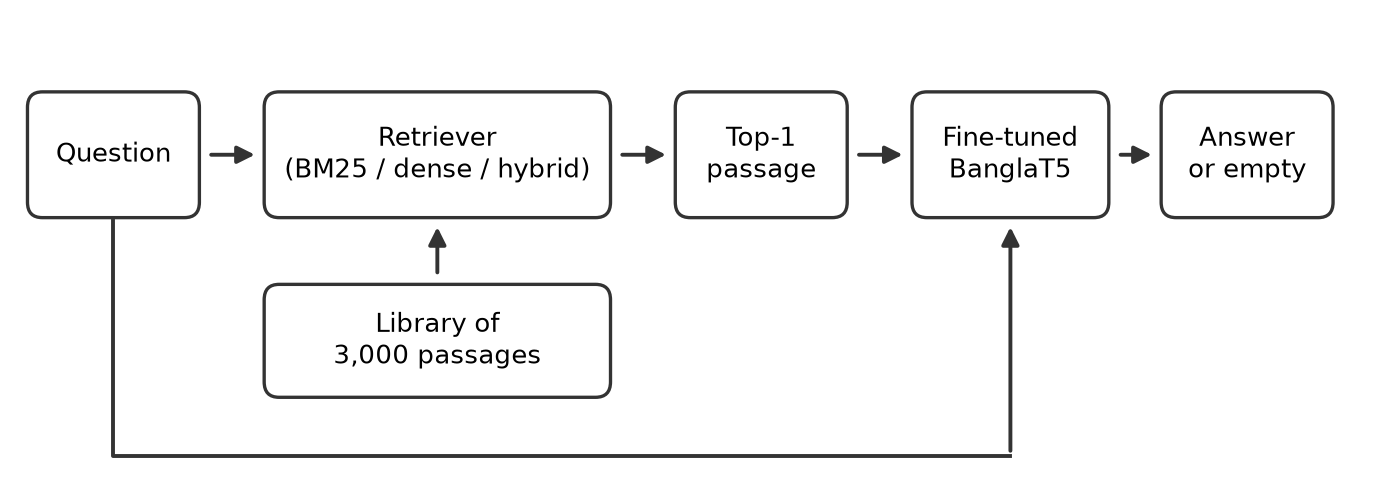
\includegraphics[width=\textwidth]{figures/pipeline.png}}{\todo{figures/pipeline.png is missing; run make\_figures.py}}
	\caption{The question-answering pipeline. The question is used twice: to search the library and as part of the input to the reader.}
	\label{fig:pipeline}
\end{figure}

\section{Dataset}

\subsection{BanglaRQA}

The system uses BanglaRQA \cite{ekram2022banglarqa}, which is released under the CC BY-NC-SA 4.0 licence. The data is downloaded when the code runs and is not shipped with it. Each of the 3,000 Wikipedia passages comes with several questions. A question has a type (factoid, causal, confirmation or list), a flag that says whether the passage answers it, and one or two reference answers. An answer is a single span, several spans separated by semicolons, or a yes/no word.

The official split is used as it is (Table~\ref{tab:split}). It is made by passage, so no passage appears in two splits. About a quarter of the questions in every split cannot be answered from their passage.

\begin{table}[H]
	\centering
	\caption{BanglaRQA splits used in this project.}
	\label{tab:split}
	\begin{tabular}{lrrr}
		\toprule
		Split & Passages & Questions & Unanswerable \\
		\midrule
		Train & 2,400 & 11,912 & 2,904 (24.4\%) \\
		Validation & 300 & 1,484 & 358 (24.1\%) \\
		Test & 300 & 1,493 & 369 (24.7\%) \\
		\bottomrule
	\end{tabular}
\end{table}

Five question ids are used twice in the test split. They belong to one passage, about the becquerel, which has ten questions attached; five of them are about the Shah Amanat Bridge and cannot be answered from that passage's text. Because of this, retrieval results are stored under the id together with the question text, and these five questions are left in the test set. They are 0.3\% of the questions.

\subsection{Preprocessing}

Question, passage and answer are all normalised with the \texttt{normalizer} package from the BanglaT5 authors, as its documentation requires. The training target is the first reference answer. For an unanswerable question the target is the empty string. If a question has two reference answers, only the first is used for training and for scoring, which is what the dataset authors do.

For the BanglaT5 tokenizer the median input (question plus passage) is 293 tokens. The input limit is 1,024 tokens, and 10 of the 11,912 training inputs reach it and are cut.

\section{The Reader: Fine-Tuned BanglaT5}

\subsection{Model}

The reader is BanglaT5 (\texttt{csebuetnlp/banglat5}) \cite{bhattacharjee2023banglat5}, an encoder-decoder Transformer with 12 layers in each half and about 247 million parameters, built on the T5 design \cite{raffel2020t5}. The encoder reads the question and the passage together and the decoder writes the answer one token at a time.

\subsection{Input and Output Format}

The tokenizer receives the question and the passage as a pair, question first. If the pair is longer than 1,024 tokens the passage is cut, never the question. The target is the normalised first reference answer, at most 256 tokens. An unanswerable question has an empty target, so the model learns to write nothing when the passage has no answer. This follows the dataset authors' published training code \cite{ekram2022banglarqa}.

\subsection{Training}

Training minimises the usual cross-entropy loss over the answer tokens. Examples of similar length are batched together so that short inputs are not padded up to the length of long ones. Weights are kept in 32-bit precision and the forward pass runs in bfloat16, because T5 models are known to overflow in 16-bit floating point. Table~\ref{tab:train-config} lists the settings.

\begin{table}[H]
	\centering
	\caption{Training configuration.}
	\label{tab:train-config}
	\begin{tabular}{ll}
		\toprule
		Setting & Value \\
		\midrule
		Optimizer & AdamW, no weight decay \\
		Learning rate & $1\times10^{-4}$, 5\% linear warmup, then linear decay \\
		Batch size & 8, with 2 accumulation steps (effective 16) \\
		Gradient clipping & 1.0 \\
		Epochs & 10 (about 7,450 updates) \\
		Precision & bfloat16 forward pass, fp32 weights \\
		Maximum input / target length & 1,024 / 256 tokens \\
		Random seed & 13 \\
		Hardware & one NVIDIA L4 GPU (Google Colab) \\
		\bottomrule
	\end{tabular}
\end{table}

After every epoch the model answers the whole validation set and the checkpoint with the best F1 is kept. The test set plays no part in any choice. The dataset authors trained for 15 epochs with batch size 2 and learning rate $5\times10^{-5}$, which is about 89,000 updates. I used a larger batch and a higher learning rate to finish in about 75 minutes, and then checked the result against their published scores.

\section{Retrieval}

\textbf{Library.} The library holds the 3,000 passages of all three splits, each kept whole under its identifier. Searching all of them, and not only the 300 test passages, makes the task harder and closer to real use.

\textbf{BM25.} The text is normalised to Unicode form NFC, Bangla digits become ASCII digits, punctuation (including the danda) is replaced by spaces, the text is lower-cased and split on spaces. There is no stemmer and no stop-word list. BM25 \cite{robertson2009bm25} then runs with the default parameters of the \texttt{rank\_bm25} package.

\textbf{Dense retrieval.} Passages and questions are embedded with BGE-M3 \cite{chen2024bgem3}, with no instruction prefix, and passages are read up to 1,024 tokens. The vectors are normalised, so the inner product is the cosine similarity, and an exact FAISS index \cite{johnson2019faiss} returns the nearest passages.

\textbf{Hybrid retrieval.} The BM25 and dense rankings (50 passages deep) are merged by reciprocal rank fusion \cite{cormack2009rrf}:
\begin{equation}
	\mathrm{RRF}(d) = \sum_{r \in \{\text{BM25},\ \text{dense}\}} \frac{1}{k + \mathrm{rank}_r(d)}, \qquad k = 60,
\end{equation}
where $\mathrm{rank}_r(d)$ is the position of passage $d$ in ranking $r$. No retriever was tuned.

In every retrieval condition the reader receives only the top-ranked passage. The retriever is also scored on its own. Hit@$n$ is the share of questions whose own passage is among the first $n$ results, and MRR is the mean of $1/\text{rank}$ of that passage in the first ten.

\section{Evaluation}

\subsection{Conditions}

The same checkpoint is run on all 1,493 test questions in the conditions of Table~\ref{tab:conditions}. The first is an upper bound. The next three show how much is lost when the passage has to be found. The last one has no passage at all and is only there to show how much the passage matters.

\begin{table}[H]
	\centering
	\caption{Evaluation conditions.}
	\label{tab:conditions}
	\begin{tabular}{ll}
		\toprule
		Condition & Passage given to the reader \\
		\midrule
		Gold & the question's own passage \\
		BM25 & top-1 passage from BM25 \\
		Dense & top-1 passage from BGE-M3 \\
		Hybrid & top-1 passage from reciprocal rank fusion \\
		None & no passage (the model was not trained for this) \\
		\bottomrule
	\end{tabular}
\end{table}

\subsection{Metrics}

Scoring follows the dataset authors' evaluation code, so the gold condition can be compared with their published numbers. Answers are lower-cased, ASCII punctuation is removed and white space is collapsed. \textbf{Exact match (EM)} is 1 if prediction and reference are equal after this and 0 otherwise. \textbf{F1} is the harmonic mean of token precision $P$ and recall $R$,
\begin{equation}
	F_1 = \frac{2PR}{P + R},
\end{equation}
with tokens being the space-separated words. For answers with several spans the spans are paired with the reference spans by an assignment that maximises F1, and the score is averaged over the larger of the two span counts, so a missing and an extra span both lower it. For an unanswerable question the prediction is correct only if it is empty. The authors' normalisation keeps the Bangla danda, so a trailing danda makes a prediction differ from the reference.

Results are given separately for answerable questions (HasAns, 1,124 questions) and unanswerable ones (NoAns, 369). The two behave differently. When retrieval returns a wrong passage, a model that writes nothing is still right on an unanswerable question. NoAns scores therefore say more about how often the model abstains than about retrieval, and HasAns is the main measure when comparing retrievers. The share of answerable questions answered with an empty string is reported as well.

Exact match is strict, and Bangla words carry suffixes, so I also report two relaxed matches on the answerable questions. They are secondary. One counts an answer as correct when its F1 is at least 0.5. The other counts it as correct when every reference span appears inside the prediction (after the same normalisation, with the danda ignored); this one favours long answers. The 0.5 cut-off is a common convention and not a standard. I chose it after noticing how far exact match falls below F1, and I did not try other cut-offs.

\subsection{Statistical Analysis}

All conditions are scored on the same questions, so comparisons are paired. For exact match, two retrievers are compared with McNemar's test in its mid-$p$ form \cite{fagerland2013mcnemar}. With $b$ questions that only the first retriever gets right and $c$ that only the second gets right, the two-sided mid-$p$ value is
\begin{equation}
	p = 2\sum_{i=0}^{m} \binom{b+c}{i}\,2^{-(b+c)} - \binom{b+c}{m}\,2^{-(b+c)}, \qquad m = \min(b, c).
\end{equation}
Confidence intervals come from a paired bootstrap with 10,000 resamples \cite{efron1979bootstrap, berg2012empirical}. About five test questions share a passage, so the resampling draws whole passages and not single questions. The three comparisons between retrievers (BM25 with dense, BM25 with hybrid, dense with hybrid) are corrected with the Holm procedure \cite{holm1979simple}. These choices follow general advice on significance testing in NLP \cite{dror2018hitchhiker}.

\subsection{Sanity Check Against Published Results}

The gold condition is compared with the dataset authors' test scores for BanglaT5 (EM 62.42, F1 78.11). Before the experiments I decided that a result within about three points of these would count as a successful reproduction. The retrieval conditions have no published baseline.

\subsection{Error Analysis}

From the gold condition and from the best retriever I drew 40 random answerable questions each whose exact match was 0 (80 in all). Each was labelled by hand with one cause (Table~\ref{tab:causes}). Retrieval misses and empty answers are labelled by the script from the passage identifiers and the prediction. The rest were labelled by me, from the reference, the prediction and the passage, so it is the judgement of one person. Two figures are reported: a strict one that counts only \emph{acceptable wording} as acceptable, and a lenient one that adds \emph{partial answer}.

\begin{table}[H]
	\centering
	\caption{Causes used to label wrong answers.}
	\label{tab:causes}
	\small
	\begin{tabular}{lp{10.5cm}}
		\toprule
		Cause & Meaning \\
		\midrule
		acceptable wording & right meaning, different wording: extra or missing words, a suffix, another list separator \\
		partial answer & correct as far as it goes, but a required part is missing \\
		wrong value & the right kind of answer, but the wrong entity, number or date \\
		unrelated span & text from the passage that does not answer the question \\
		yes/no flipped & a confirmation question answered with the opposite word \\
		false abstention & empty answer although the passage contains the answer \\
		retrieval miss & the wrong passage was retrieved \\
		dataset issue & the reference is wrong or ambiguous, or the answer is not in the passage \\
		\bottomrule
	\end{tabular}
\end{table}

\section{Demonstration Interface}

To show the system working, the retriever and the reader are wrapped in a small web page built with Gradio. The user types a Bangla question and picks BM25, dense or hybrid retrieval. The page shows the answer, the passage the model read, and the three best passages with their scores. When the model writes nothing, the page says that no answer was found in the retrieved passage. It runs inside the Colab notebook and is not published on the web.

\chapter{Results}

\section{Retrieval Quality}

On the full sample of 200 questions, the passage that contains the answer was among the top three retrieved chunks for 98.0\% of questions with BM25, 96.0\% with dense retrieval and 99.0\% with the hybrid method (Table~\ref{tab:rq1-metrics}). A reference answer appeared verbatim in the retrieved text for only 73--75\% of questions. The gap of more than 20 points between finding the right passage and having the answer string in the retrieved chunks suggests that the 512-character chunking, not passage finding, limits what the generator can use. (Some answers are paraphrases and would not match as an exact string, so the second number is a lower bound on whether the answer was available.)

\section{RQ1: Effect of Retrieval Method on Answer Accuracy}

Table~\ref{tab:rq1-metrics} shows the metrics for each setting, and Table~\ref{tab:rq1-mcnemar} shows paired tests against the no-retrieval baseline.

\begin{table}[H]
	\centering
	\caption{Answer metrics per setting (mean and 95\% bootstrap CI).}
	\label{tab:rq1-metrics}
	\IfFileExists{tables/rq1_metrics.tex}{\resizebox{\textwidth}{!}{%
\begin{tabular}{lcccccc}
\toprule
\textbf{Setting} & \textbf{n} & \textbf{EM} & \textbf{F1} & \textbf{Correct (F1>=0.5)} & \textbf{Passage hit@3} & \textbf{Answer in context} \\
\midrule
no retrieval & 200 & 0.150 [0.100, 0.200] & 0.269 [0.218, 0.324] & 0.280 [0.220, 0.345] & - & - \\
BM25 & 200 & 0.425 [0.355, 0.490] & 0.739 [0.694, 0.779] & 0.830 [0.775, 0.880] & 0.980 [0.960, 0.995] & 0.745 [0.680, 0.805] \\
dense (BGE-M3) & 200 & 0.410 [0.340, 0.475] & 0.740 [0.698, 0.781] & 0.855 [0.800, 0.900] & 0.960 [0.930, 0.985] & 0.730 [0.670, 0.790] \\
hybrid (BM25 + BGE-M3) & 200 & 0.440 [0.370, 0.505] & 0.754 [0.711, 0.793] & 0.840 [0.790, 0.890] & 0.990 [0.975, 1.000] & 0.750 [0.690, 0.810] \\
\bottomrule
\end{tabular}%
}
}{\todo{run make\_tables.py to create tables/rq1\_metrics.tex}}
\end{table}

\begin{table}[H]
	\centering
	\caption{Paired McNemar tests against the no-retrieval baseline (correct means F1 $\ge$ 0.5; Holm-adjusted).}
	\label{tab:rq1-mcnemar}
	\IfFileExists{tables/rq1_mcnemar.tex}{\resizebox{\textwidth}{!}{%
\begin{tabular}{lcccccc}
\toprule
\textbf{Setting} & \textbf{paired n} & \textbf{better than none only} & \textbf{worse only} & \textbf{diff (acc)} & \textbf{p (exact)} & \textbf{p (Holm)} \\
\midrule
BM25 & 200 & 111 & 1 & 0.550 & 0.000 & 0.000 \\
dense (BGE-M3) & 200 & 117 & 2 & 0.575 & 0.000 & 0.000 \\
hybrid (BM25 + BGE-M3) & 200 & 113 & 1 & 0.560 & 0.000 & 0.000 \\
\bottomrule
\end{tabular}%
}
}{\todo{run make\_tables.py to create tables/rq1\_mcnemar.tex}}
\end{table}

Retrieval helps a great deal. With no retrieval, only 28.0\% of answers were correct (F1 $\ge$ 0.5; 95\% CI 22.0--34.5) and exact match was 15.0\%. All three retrieval settings reach 83--86\% correct, a gain of 55 to 57.5 percentage points over the baseline. The paired tests agree: against the no-retrieval baseline, BM25 fixed 111 questions and broke 1, dense retrieval fixed 117 and broke 2, and the hybrid method fixed 113 and broke 1 (all Holm-adjusted $p < 0.0001$).

The three retrievers cannot be separated on this sample. Their correct rates are 83.0\% (BM25), 85.5\% (dense) and 84.0\% (hybrid) with overlapping confidence intervals (for example 77.5--88.0 for BM25 and 80.0--90.0 for dense). Against the dense default, BM25 was better on 6 questions and worse on 11 (difference $-2.5$ points, Holm-adjusted $p = 0.66$), and the hybrid method was better on 5 and worse on 8 ($p = 0.66$). The hybrid method had the highest passage hit rate (99.0\%) and the highest exact match (44.0\%), but these differences are within the confidence intervals. With 200 questions the study can detect a large effect such as retrieval versus none, but not a difference of a few points between retrievers, so the honest conclusion is that no retriever is shown to be better than another.

\section{RQ2: RAGAS Compared with Human Grades}

\textbf{Random answers have no variance to measure.} On the first 100 randomly sampled answers, 98 faithfulness grades were 3, and RAGAS faithfulness showed no correlation with them ($\rho \approx 0$, with a very narrow interval, which is what a ceiling effect looks like). Answer relevance was similarly uninformative. This is why the graded set was extended with likely-bad, closed-book and synthetic unsupported answers (Section~\ref{sec:method-rq2}).

\textbf{Detection of unsupported answers.} On the final 290 graded answers (220 supported, 69 unsupported, one without a score), RAGAS faithfulness with English judge prompts and Gemini as judge ranks unsupported answers below supported ones with an AUC of 0.909 (95\% CI 0.866--0.944). Using a threshold of 0.5, it flags 89.9\% of unsupported answers, but also 9.1\% of supported answers. The AUC is 0.955 on the 30 synthetic rows and 0.875 on the 39 natural unsupported rows (closed-book and low-F1 answers); the natural figure is the fairer estimate of performance on real RAG output. Supported answers had a mean faithfulness of 0.907.

\textbf{Correlation.} Spearman's $\rho$ between RAGAS faithfulness and the faithfulness grade is 0.782 (95\% CI 0.700--0.853, $n = 289$). This is high but should not be read as agreement on ordinary answers: the sample deliberately mixes good and bad answers, which inflates a rank correlation. For answer relevance, $\rho = 0.294$ (0.167--0.398, $n = 285$). Only 13 of 290 answers have a relevance grade below 3, most of them refusals, so this estimate rests on very few informative rows, and RAGAS answer relevancy cannot be recommended as a stand-in for a grade here.

\textbf{Prompt language.} \todo{Insert the Bangla-prompt result when the run is finished (AUC and false-alarm rate for judge prompts adapted to Bengali, scored on N rows), or state that it could not be completed. Note that RAGAS' automatic prompt translation failed on its first attempt with this judge model and succeeded on a retry.}

\section{Discussion}

For a practitioner, two things follow. First, retrieval is the large effect: any of the three retrievers more than triples the share of correct Bangla answers over asking the model alone, and choosing among BM25, dense and hybrid matters much less than whether the retrieved text actually contains the answer (about a quarter of questions did not have the answer string in the top three chunks even when the right passage was found). Second, an English-prompted RAGAS faithfulness score is a usable screening tool for unsupported Bangla answers, with an AUC around 0.9, but it is not a clean pass/fail test: it flags roughly one in eleven good answers, so flagged answers need a look rather than automatic rejection.

The results are uncertain in several places: the retrievers are not separated, the unsupported examples are few (69, of which 30 are synthetic), and the reference grades are AI-drafted and author-reviewed (Chapter~5).

\chapter{Conclusion and Future Work}

\section{Conclusion}

\todo{Write after the results are final. State the answer to RQ1 and RQ2 in two or three sentences each, with the key numbers and their confidence intervals.}

\section{Limitations}

\begin{itemize}
	\item \textbf{Domain change.} The planned medical-textbook corpus was replaced by general-domain Bangla Wikipedia (BanglaRQA), so results may not carry over to medical text.
	\item \textbf{Possible training exposure.} The generator may have seen Wikipedia text during training; the no-retrieval baseline measures this, but cannot remove it.
	\item \textbf{One dataset and one generator.} Findings describe this dataset and this model family, not Bangla RAG in general.
	\item \textbf{Sample size.} With a few hundred questions, and about 100 human-graded answers, confidence intervals are wide, so small differences between settings cannot be resolved.
	\item \textbf{One factor at a time.} Retrieval method was varied with chunk size and number of chunks held fixed, so interactions between them are not measured.
	\item \textbf{Judge and generator from the same family.} Gemini both generates and judges, which may bias the RAGAS scores toward the generator.
	\item \textbf{Literature search.} The search was web-based; ``no prior study found'' statements should be checked against Google Scholar and Semantic Scholar.
\end{itemize}

\section{Future Research Directions}

\begin{itemize}
	\item Repeat the study on the original medical-textbook corpus if the text becomes available.
	\item Vary chunk size, number of retrieved chunks and the embedding model, including a Bengali sentence encoder and multilingual E5.
	\item Add a second, independent judge model, and a second human grader to measure human--human agreement.
	\item Test open-weight generators, to see whether the findings hold outside one commercial model family.
\end{itemize}


% ============================ REFERENCES ============================
\clearpage
\addcontentsline{toc}{chapter}{\numberline{}References}
\printbibliography[title={References}]

\end{document}
